\begin{figure*}
\begin{center}
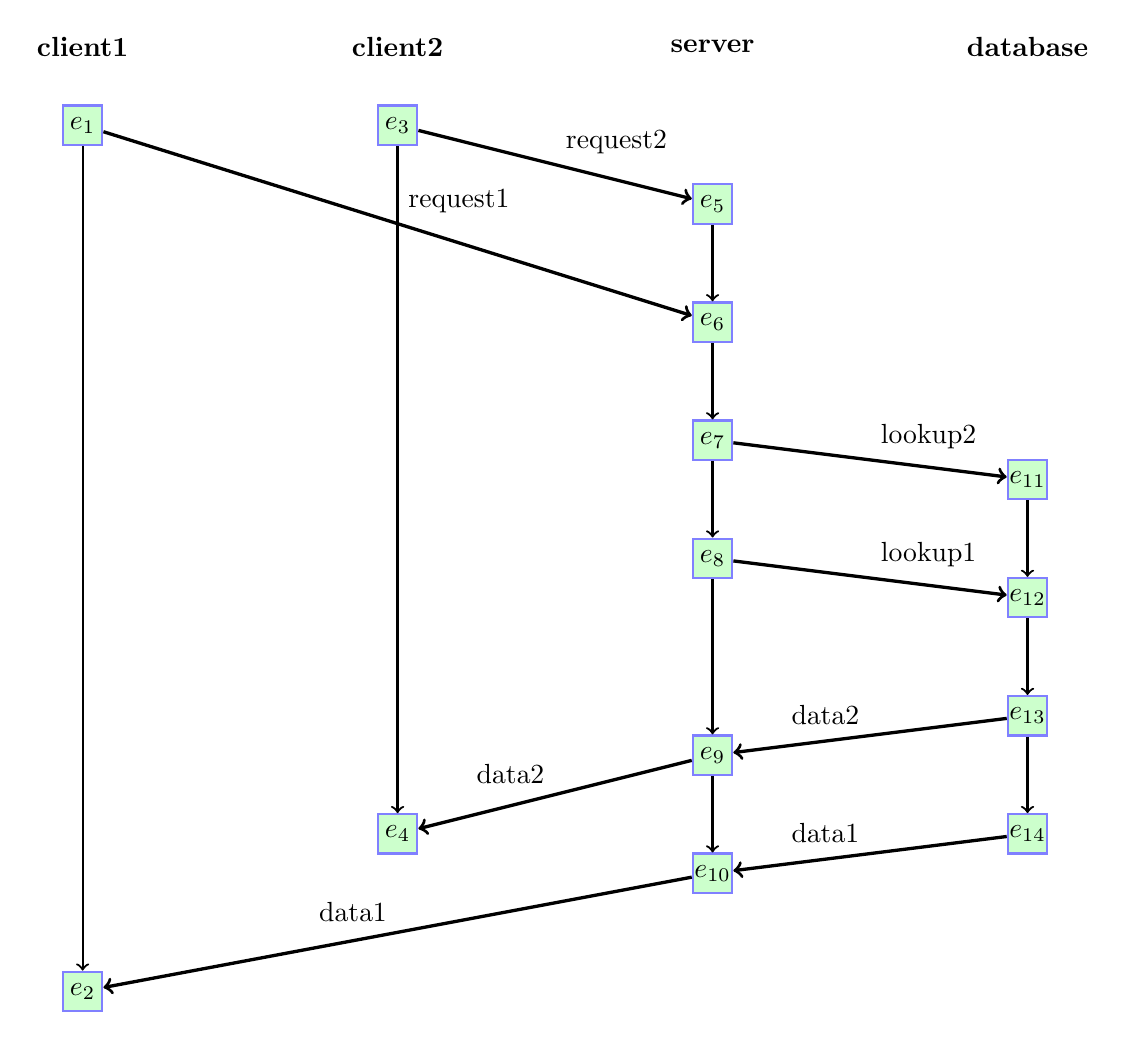
\begin{tikzpicture}{scale=0.6}
	\node 			at	(-8,7) 	[rectangle, thick]{\textbf{client1}};
	\node 			at	(-4,7) 	[rectangle, thick]{\textbf{client2}};
	\node 			at	(0,7) 	[rectangle, thick]{\textbf{server}};
	\node 			at	(4,7) 	[rectangle, thick]{\textbf{database}};


	\node 	(e1)		at	(-8,6) 	[rectangle, thick, draw=blue!50,fill=green!20,inner sep=0pt,minimum size=.50cm]{$e_1$};


	\node 	(e2)		at	(-8,-5) 	[rectangle, thick, draw=blue!50,fill=green!20,inner sep=0pt,minimum size=.50cm]{$e_2$};


	\node 	(e3)		at	(-4,6) 	[rectangle, thick, draw=blue!50,fill=green!20,inner sep=0pt,minimum size=.50cm]{$e_3$};


	\node 	(e4)		at	(-4,-3) 	[rectangle, thick, draw=blue!50,fill=green!20,inner sep=0pt,minimum size=.50cm]{$e_4$};


	\node 	(e5)		at	(0,5) 	[rectangle, thick, draw=blue!50,fill=green!20,inner sep=0pt,minimum size=.50cm]{$e_5$};


	\node 	(e6)		at	(0,3.5) 	[rectangle, thick, draw=blue!50,fill=green!20,inner sep=0pt,minimum size=.50cm]{$e_6$};


	\node 	(e7)		at	(0,2) 	[rectangle, thick, draw=blue!50,fill=green!20,inner sep=0pt,minimum size=.50cm]{$e_7$};


	\node 	(e8)		at	(0,0.5) 	[rectangle, thick, draw=blue!50,fill=green!20,inner sep=0pt,minimum size=.50cm]{$e_8$};

	\node 	(e9)		at	(0,-2) 	[rectangle, thick, draw=blue!50,fill=green!20,inner sep=0pt,minimum size=.50cm]{$e_9$};


	\node 	(e10)		at	(0,-3.5) 	[rectangle, thick, draw=blue!50,fill=green!20,inner sep=0pt,minimum size=.50cm]{$e_{10}$};


	\node 	(e11)		at	(4,1.5) 	[rectangle, thick, draw=blue!50,fill=green!20,inner sep=0pt,minimum size=.50cm]{$e_{11}$};


	\node 	(e12)		at	(4,0) 	[rectangle, thick, draw=blue!50,fill=green!20,inner sep=0pt,minimum size=.50cm]{$e_{12}$};


	\node 	(e13)		at	(4,-1.5) 	[rectangle, thick, draw=blue!50,fill=green!20,inner sep=0pt,minimum size=.50cm]{$e_{13}$};


	\node 	(e14)		at	(4,-3) 	[rectangle, thick, draw=blue!50,fill=green!20,inner sep=0pt,minimum size=.50cm]{$e_{14}$};

	\draw[->, thick]	(e1)	to	node[auto]{}	(e2);

	\draw[->, thick] 	(e3) 	to 	node[auto]{} 	(e4);

	\draw[->, thick]	(e5)	to	node[auto]{}	(e6);
	\draw[->, thick] 	(e6) 	to 	node[auto]{} 	(e7);
	\draw[->, thick]	(e7)	to	node[auto]{}	(e8);
	\draw[->, thick] 	(e8) 	to 	node[auto]{} 	(e9);
	\draw[->, thick]	(e9)	to	node[auto]{}	(e10);

	\draw[->, thick] 	(e11) 	to 	node[auto]{} 	(e12);
	\draw[->, thick] 	(e12) 	to 	node[auto]{} 	(e13);
	\draw[->, thick] 	(e13) 	to 	node[auto]{} 	(e14);


	\draw[->,very thick] (e1) to 	node[auto]{request1} 		(e6);
	\draw[->,very thick] (e3) to 	node[auto]{request2} 		(e5);

	\draw[->,very thick] (e7) to 	node[auto]{lookup2} 		(e11);
	\draw[->,very thick] (e8) to 	node[auto]{lookup1} 		(e12);

	\draw[->,very thick] (e13) to 	node[auto,swap]{data2} 		(e9);
	\draw[->,very thick] (e9) to 	node[auto,swap]{data2} 		(e4);

	\draw[->,very thick] (e14) to 	node[auto,swap]{data1} 		(e10);
	\draw[->,very thick] (e10) to 	node[auto,swap]{data1} 		(e2);

\end{tikzpicture}
\end{center}
\caption{Lamport diagram representing a scenario of client-server  system}
\label{fig:client-server-ld}
\end{figure*}
